\pagestyle{fancy}
%%%%%%%%%%%%%%%%% FAIR
\section{FAIR}\thispagestyle{fancy}
FAIR (\emph{Facility for Antiproton and Ion Research}) \cite{fair} is an international accelerator facility for the research with antiprotons and ions which is being developed and built in cooperation with international partners, i.a. Poland. FAIR is being built at the GSI Helmholtzzentrum für Schwerionenforschung in Darmstadt, Germany. The existing GSI accelerators will become part of the future FAIR facility and serve as the first acceleration stage \cite{fair}. The new accelerator, SIS 100, is  foreseen to become
operational in 2025 \cite{progress report}. The map of the existing facilities of GSI, and FAIR (which is still under construction) is shown on Figure \ref{fair map}. Several experiments will be held at FAIR: APPA, HADES, NUSTAR, PANDA, and CBM.
\begin{figure}[H]
    \centering
    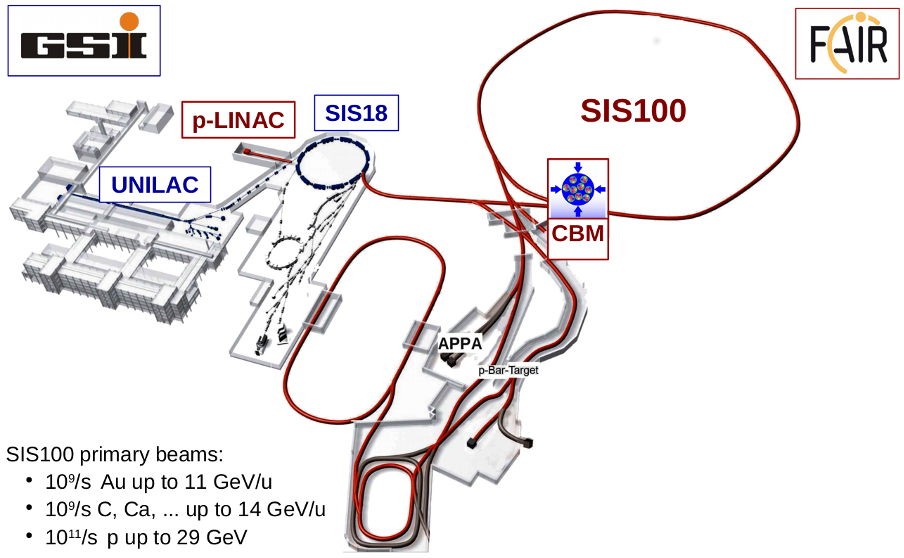
\includegraphics[width=.7\textwidth]{img/fair map.png}
    \caption{Map of FAIR\cite{fair}}
    \label{fair map}
\end{figure}
%%%%%%%%%%%%%%%%%%%%%%%%%%%% CBM
\section{CBM experiment}
The CBM experiment will be held at the Facility for Antiproton and Ion Research. Its goal is the exploration of the QCD phase diagram in the region of high net baryon densities and moderate temperatures. It will allow i.a. studying the equation-of-state of nuclear matter at neutron star core densities. The measurements will be performed at reaction rates up to 10 MHz. It requires a highly efficient particle identification and reconstruction framework. \cite{cbm-experiment}
%%%%%%%%%%%%%%%%%%%%% CBM SETUP
\subsection{CBM setup}
In order to identify the particles coming from the collisions, the setup of 8 detectors is under development in FAIR (Figure \ref{cbm_setup}).
\begin{figure}[H]
    \centering
    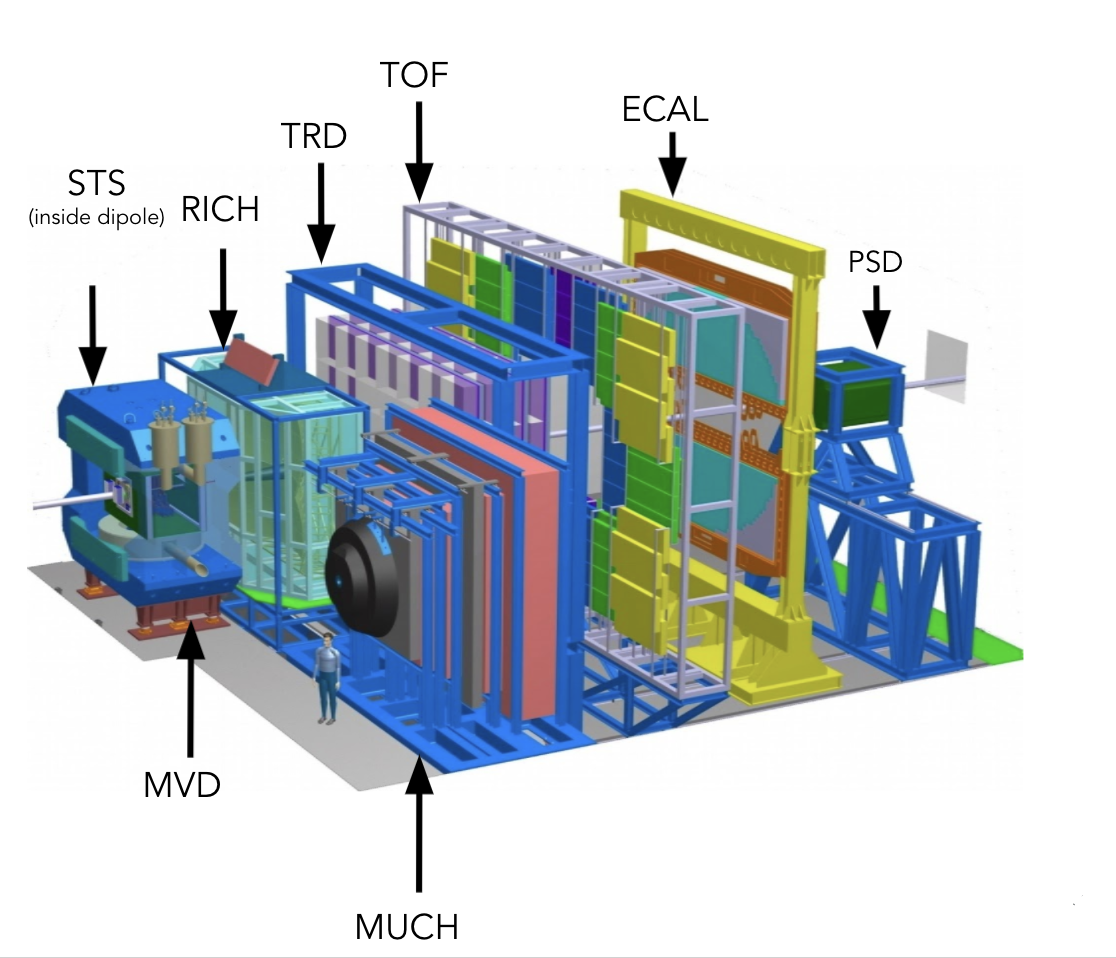
\includegraphics[width=.7\textwidth]{img/cbm_setup.png}
    \caption{CBM setup \cite{progress report}}
    \label{cbm_setup}
\end{figure}
The CBM detectors setup will consist of \cite{progress report}:
\begin{itemize}
    \item STS - Silicon Tracking System
    \item MVD - Micro Vertex Detector
    \item RICH - Ring Imaging Cherenkov Detector, replaceable with:
    \item MUCH - Muon Chamber System
    \item TRD - Transition Radiation Detector
    \item TOF - Time of Flight Detector
    \item ECAL - Electromagnetic Calorimeter
    \item PSD - Projectile Spectator Detector.
\end{itemize}

%%%%%%%%%%%%%%%%%%%Theoretical models
\subsection{Monte Carlo models}
As the main CBM accelerator, the SIS100, will not start functioning earlier than in 2025, the Monte Carlo models are handy in simulating the possible results and planning the actual setup of the experiment \cite{progress report}.

The majority of the simulations performed by the CBM Collaboration are performed using two Monte Carlo-based simulation packages: \textbf{URQMD} (Ultra relativistic Quantum Molecular Dynamics) \cite{urqmd}, and \textbf{DCM-QGSM-SMM} (Dubna Cascade Model and Statistical Multifragmentation Model) \cite{dcm}. Both models  treat the production of new particles via the formation and fragmentation of specific colored objects, strings. The differences between the models arise on different stages of a string formation and fragmentation. \cite{dcm}
 A heavy-ion collision is visualised on Figure \ref{urqmd}.

\begin{figure}[H]
    \centering
    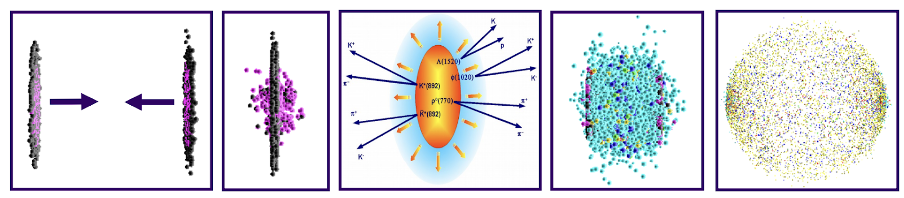
\includegraphics[width=.9\textwidth]{img/urqmd.png}
    \caption{Visualisation of heavy-ion collisions in the URQMD model\cite{slodkowski}}
    \label{urqmd}
\end{figure}

The data from the Monte Carlo models is later passed through \textbf{GEANT4} - a toolkit for simulating the passage of particles through matter \cite{geant4}. The CBM setup is simulated in it, allowing to recreate the behaviour and work of different detectors and the influence of the construction elements. Finally, the simulated MDV, STS, RICH, TDR, TOF, and PSD hits are reconstructed into tracks and clusters and processed into a special data format, called \emph{Analysis Tree} \cite{atree}.


